\vspace*{1em}

{\bf \large Numbers.} For the purposes of this class, following number systems are the ones we care for:
\begin{itemize}
\item \textbf{Natural numbers}, $\nn = \set{0,1,2,\ldots}$.\\[0.5em]
Our natural numbers will include $0$, and therefore will have a neutral element for both addition and multiplication.
\item \textbf{Integers}, $\zz = \set{\ldots,-2,-1,0,1,2,\ldots}$.\\[0.5em]
The "Z" comes from \emph{Zahlen}, which is the German word for number.\\[0.5em]
We will denote the set of positive integers as $\zz_+ = \set{1,2,3,\ldots}$.
\item \textbf{Rational numbers}, $\qq = \setp{\dfrac{a}{b}}{a,b \in \zz,\,b \neq 0}$.\\[0.5em]
The "Q" stands for quotient.
\item \textbf{Real numbers}, $\rr$ are numbers with a decimal representation. $\rr$ is made up of $\qq$ and the set of, so-called, irrational numbers. Even amongst irrational numbers, we can make a distinction: numbers such as $\sqrt{2}$ that are solutions to polynomial equations ($x^2 - 2 = 0$) and numbers like $\pi$ which are not. The former are called \emph{algebraic numbers} and much of field and Galois theory can be used to study them carefully, the latter are called \emph{transcendental numbers}.\\[0.5em]
$\rr$ is just one of many "jumps" one can make from $\qq$, there are more (indexed by prime numbers), that are treated in advanced number theory, called the $p$-adic numbers, denoted $\qq_p$.
\item \textbf{Complex numbers}, $\cc = \setp{a + bi}{a,b \in \rr,\,i^2 = -1}$.\\[0.5em]
Complex numbers are an "algebraic jump" from the real numbers since $i$ is a solution to the polynomial equation $x^2 + 1 = 0$.
\end{itemize}

\vspace{2em}

{\bf\large Questions in Number Theory.} Number Theory, more than any other field in mathematics, is defined by the questions it entails; more often than this subject is context. The kinds of questions one asks are as follows
\begin{itemize}
\item \textbf{involving polynomial equations}
\begin{itemize}
\item[$\triangleright$] does the polynomial equation $2x - 1 = 0$ have an integer solution?\\[0.2em]
\emph{Ans}. No, this is equivalent to $1/2 \notin \zz$.
\item[$\triangleright$] does the polynomial equation $x^2 + y^2 = 1$ have a rational solution?\\[0.2em]
\emph{Ans}. Yes, this is related to a discussion on Pythagorean triplets and the unit circle.
\item[$\triangleright$] On the application front, Elliptic Curve Cryptography is of this nature.
\end{itemize}
\item \textbf{involving prime numbers}
\begin{itemize}
\item[$\triangleright$] counting prime numbers.\\[0.2em]
A result of paramount importance here is the \emph{Prime Number Theorem}.
\item[$\triangleright$] On the application front, the RSA cryptosystem is of this nature.
\end{itemize}
\item \textbf{square a circle}: can there be a square whose area is $\pi$?\\[0.2em]
\emph{Ans}. No! This is related to the notion of transcendence and constructibility.
\end{itemize}

\vspace*{2em}

\begin{center}
{\Large The (Euclidean) Division Algorithm}
\end{center}

{\bf\large Linear Diophantine Equations.}
Let's pose a geometric question: in the euclidean plane, consider the integer grid and a line with rational slope and rational $y$-intercept
\[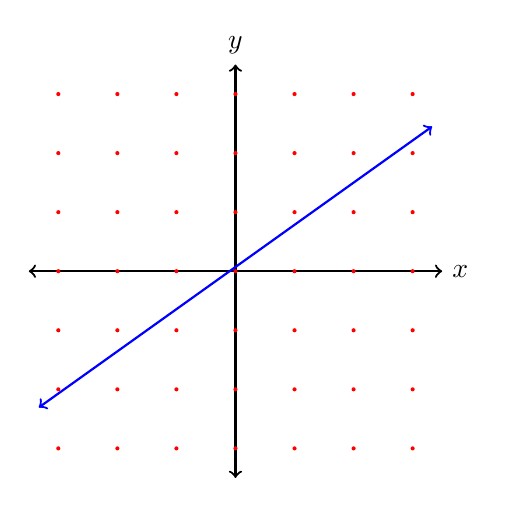
\begin{tikzpicture}[scale=0.75]
    \draw[<->,thick] (-3.5,0)--(3.5,0) node[right]{$x$};
	\draw[<->,thick] (0,-3.5)--(0,3.5) node[above]{$y$};
    \foreach \x in {-3,-2,-1,0,1,2,3}
    \foreach \y in {-3,-2,-1,0,1,2,3}
    {
    \fill[red] (\x,\y) circle (1pt);
    }
    \draw[<->,blue,thick] (-3.33,-2.307) -- (3.33,2.45);
  \end{tikzpicture}\]
Does it intersect the integer grid?\\
\\
Algebraically, let $A,B,C \in \zz$, does there exist $(x,y) \in \zz^2$ such that
\[Ax + BY = C\]

\vspace*{0.5em}

\emph{\textbf{Question}}. \textit{Can we find $(x,y) \in \zz^2$ such that $133x + 85y = 1$?}\\[0.5em]
\emph{\textbf{Discussion}}. Visually, what we're asking for is this: suppose you are standing at $0$ on the number line and you're allowed to
\begin{itemize}
\item \emph{\color{blue} hop} 133 steps left (-133) or right (+133)
\item \emph{\color{red} skip} 85 steps left (-85) or right (+85)
\end{itemize}
\vspace*{1em}
\[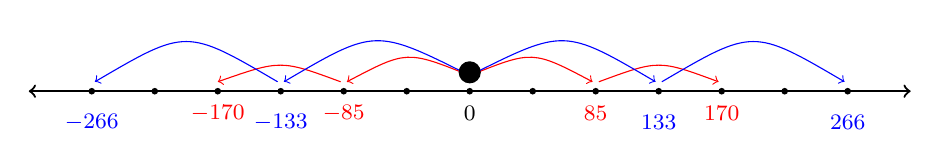
\begin{tikzpicture}[scale=0.8]
    \draw[<->,thick] (-7,0)--(7,0);
	\foreach \x in {-6,-5,-4,-3,-2,-1,0,1,2,3,4,5,6}
    {
    \fill (\x,0) circle (1.5pt);
    }
    \node[] at (0,-0.35) {\footnotesize$0$};
    \node[] at (2,-0.35) {\footnotesize\color{red}$85$};
    \node[] at (4,-0.35) {\footnotesize\color{red}$170$};
    \node[] at (-2,-0.35) {\footnotesize\color{red}$-85$};
    \node[] at (-4,-0.35) {\footnotesize\color{red}$-170$};
    \node[] at (3,-0.5) {\footnotesize\color{blue}$133$};
    \node[] at (6,-0.5) {\footnotesize\color{blue}$266$};
    \node[] at (-3,-0.5) {\footnotesize\color{blue}$-133$};
    \node[] at (-6,-0.5) {\footnotesize\color{blue}$-266$};
    \draw[red,->] (0,0.25) .. controls (1,0.65) .. (1.95,0.15);    
    \draw[red,->] (2.05,0.15) .. controls (3,0.5) .. (3.95,0.15);    
    \draw[red,->] (0,0.25) .. controls (-1,0.65) .. (-1.95,0.15);    
    \draw[red,->] (-2.05,0.15) .. controls (-3,0.5) .. (-4,0.15);    
    \draw[blue,->] (0,0.25) .. controls (1.5,1) .. (2.95,0.15);    
    \draw[blue,->] (3.05,0.15) .. controls (4.5,1) .. (5.95,0.15);    
    \draw[blue,->] (0,0.25) .. controls (-1.5,1) .. (-2.95,0.15);    
    \draw[blue,->] (-3.05,0.15) .. controls (-4.5,1) .. (-5.95,0.15);    
    \fill[] (0,0.3) circle (0.5em);
	\end{tikzpicture}\]
Then we want to know if you can hop $x$-many times and skip $y$-many times to get to $1$. For example, hopping twice to the right and skipping thrice to the left gets you
\[133\cdot (+2) + 85\cdot (-3) = 266 - 255 = 11\]
%\newpage
The answer is \textbf{yes}. The theoretical reason is the $\gcd$, \emph{greatest common divisor}, and the algorithmic reason is the \emph{(Euclidean) Division Algorithm}.

\vspace*{2em}

{\bf \large (Euclidean) Division Algorithm.}
The purpose is to check if $Ax + By = C$ has any integer solution and to find them all.
\begin{itemize}
\item Start with two positive integers $a,b$, assume $a \geq b$.
\item Divide $a$ by $b$
\[a = bq + r,\quad 0 \leq r < b,\quad q \in \zz\]
\item If $r = 0$, \textsl{halt}. If not, repeat the previous steps by replacing $(a,b)$ by $(b,r)$.
\item Continue until your remainder is $0$, this process will terminate in finite steps.
\end{itemize}
%In haiku,
%\begin{center}
%{\footnotesize
%Divisor to front,\\
%remainder to divisor,\\
%ignore the quotient.
%}
%\end{center}

\vspace*{1em}

Let's revisit the equation above, and see how the algorithm above makes it possible for us to find a required solution.
\begin{example}\label{example 1}
Employ the Division Algorithm to $(133,85)$ and find a solution to the equation $133x + 85y = 1$.
\end{example}
\begin{proof}[Answer]
Let's employ the Division Algorithm
\begin{align*}
{\color{blue} 133} &= {\color{blue} 85}\cdot (1) + {\color{red} 48}\\[0.5em]
{\color{blue} 85} &= {\color{blue} 48}\cdot (1) + {\color{red} 37}\\[0.5em]
{\color{blue} 48} &= {\color{blue} 37}\cdot (1) + {\color{red} 11}\\[0.5em]
{\color{blue} 37} &= {\color{blue} 11}\cdot (3) + {\color{red} 4}\\[0.5em]
{\color{blue} 11} &= {\color{blue} 4}\cdot (2) + {\color{red} 3}\\[0.5em]
{\color{blue} 4} &= {\color{blue} 3}\cdot (1) + {\color{red} 1}\\[0.5em]
{\color{blue} 3} &= {\color{blue} 1}\cdot (3) + {\color{red} 0}
\end{align*}
Let's take the last non-zero remainder, $1$, and work backwards in the following fashion
\begin{align*}
1 &= 4 + {\color{red} 3}\cdot (-1)\\[0.5em]
&= 4 + {\color{red} (11 - 4\cdot(2))}\cdot (-1)\\[0.5em]
&= 11\cdot (-1) + {\color{red} 4}\cdot (3)\\[0.5em]
&= 11\cdot (-1) + {\color{red} (37 - 11\cdot(3))}\cdot (3)\\[0.5em]
&= 37\cdot (3) + {\color{red} 11}\cdot (-10)\\[0.5em]
&= 37\cdot (3) + {\color{red} (48 - 37\cdot(1))}\cdot (-10)\\[0.5em]
&= 48\cdot (-10) + {\color{red} 37}\cdot (13)\\[0.5em]
&= 48\cdot (-10) + {\color{red} (85 - 48\cdot (1))}\cdot (13)\\[0.5em]
&= 85\cdot (13) + {\color{red} 48}\cdot (-23)\\[0.5em]
&= 85\cdot (13) + {\color{red} 133 - 85\cdot (1)}\cdot (-23)\\[0.5em]
&= 133\cdot ({\color{blue} -23}) + 85\cdot({\color{blue} 36})
\end{align*}
Therefore $(x,y) = (-23,36)$ is such that $133x + 85y = -3059 + 3060 = 1$.
\end{proof}

%\vspace*{1em}

\begin{example}
Does there exist a solution to the equation $91x + 49y = 1$.
\end{example}
\begin{proof}[Answer]
Let's employ the Division Algorithm as we did in the previous example
\begin{align*}
{\color{blue} 91} &= {\color{blue} 49}\cdot (1) + {\color{red} 42}\\[0.5em]
{\color{blue} 49} &= {\color{blue} 42}\cdot (1) + {\color{red} 7}\\[0.5em]
{\color{blue} 42} &= {\color{blue} 7}\cdot (6) + {\color{red} 0}
\end{align*}
Unlike the previous example where the last non-zero remainder was exactly the number on the right hand side of the given equation, we have $7$ which is not the number on the right hand side of the given equation, $1$. So, one may guess that this equation doesn't have a solution.\\
\\
One would then be correct, let's show this by way of contradiction. Suppose there did exist a pair $(x,y) \in \zz^2$ such that $91x + 49y = 1$, which gives us
\[7\cdot (13x + 7y) = 1.\]
This tells us that $7 \mid 1$ ($7$ divides $1$), which is preposterous. Therefore no solution exists.
\end{proof}

It would have been a different story if the right hand side was divisible by $7$, which happens to be $\gcd(91,49)$ and the last non-zero remainder we obtained using the division algorithm. This is not a coincidence.

\vspace*{1.5em}

\begin{remark}
The fact that the equation $133x + 85y = 1$ has a solution $(x,y) = (-23,36)$ means that $133x + 85y = c$ has a solution for any integer $c$, which is nothing but $(-23c,36c)$.
\end{remark}

\vspace*{1em}

\begin{definition}[Greatest Common Divisor]
Let $a,b$ be non-zero integers, than any positive integer $g$ is called a \emph{greatest common denominator} of $a$ and $b$, denoted $\gcd(a,b)$ or $\gcd(b,a)$, if
\begin{itemize}
\item[(D1)] $g\mid a$ and $g\mid b$, i.e. if $g$ is a common divisor; and
\item[(D2)] $d$ is any integer such that $d\mid a$ and $d\mid b$, then $d\mid g$.
\end{itemize}
\vspace{0.5em}
\emph{e.g.} $\gcd(-4,6) = 2,\ \gcd(91,49) = 7,\ \gcd(133,85) = 1$
\end{definition}

\vspace*{1em}

\begin{lemma}
The $\gcd$ for a given pair of non-zero integers is unique.
\end{lemma}
\begin{proof}
Let $a,b$ be non-zero integers and suppose $g$ and $g'$ are two $\gcd$'s of $a$ and $b$. In particular, both of them are common divisors of $a$ and $b$, therefore by (D2) we have $g\mid g'$ and $g'\mid g$. Hence $g = g'$, since $g,g'>0$ (see Problem \ref{div a}); thus, the $\gcd$ is unique.
\end{proof}

\vspace*{1em}

\begin{theorem}\label{Theorem 1.6}
Let $a,b$ be positive integers. The last non-zero remainder $R$ obtained under the Division Algorithm applied to $a$ and $b$ is equal to $\gcd(a,b)$.
\end{theorem}
\begin{proof}
To prove this theorem, we will first prove the following lemma\\
\begin{subproof}
\vspace*{-0.1in}
\begin{lemma}\label{Lemma 1.7}
Let $u,v,q,r$ be integers such that $u = vq + r$, then
\[g = \gcd(u,v) \iff g = \gcd(v,r)\]
\end{lemma}
\begin{proof}
($\Rightarrow$) Suppose $g = \gcd(u,v)$, let's prove $g = \gcd(v,r)$.
\begin{itemize}
\item[(i)] Since $g = \gcd(u,v)$, therefore $g\mid u$ and $g\mid v$. Since $u = vq + r$, hence $r = u - vq$ and thus $g\mid r$ (see Problem \ref{div a}). Therefore $g\mid v$ and $g\mid r$.
\item[(ii)] Let $d\mid v$ and $d\mid r$, then since $u = vq + r$, we have $d\mid u$. That is, $d\mid u$ and $\mid v$, and since $g = \gcd(u,v)$, by definition $g\mid d$.
\end{itemize}
By definition, we then have $g = \gcd(v,r)$. A very similar argument gives you ($\Leftarrow$).
\end{proof}
\vspace*{0.01em}
\end{subproof}
\vspace*{0.5em}
With this lemma in mind, let's assume, without loss of generality, $a\geq b$. We employ the Division Algorithm and let's assume it terminates in $n$ steps, that is our algorithm gives us the following
\begin{align*}
a &= bq_1 + r_1 & \text{(Step 1)}\\[0.25em]
b &= r_1q_2 + r_2 & \text{(Step 2)}\\[0.25em]
r_1 &= r_2q_3 + r_3 & \text{(Step 3)}\\[0.25em]
&\quad\vdots\\[0.25em]
r_{n-4} &= r_{n-3}q_{n-2} + r_{n-2} & \text{(Step $n-2$)}\\[0.25em]
r_{n-3} &= r_{n-2}q_{n-1} + R & \text{(Step $n-1$)}\\[0.25em]
r_{n-2} &= Rq_n + 0 & \text{(Step $n$)}
\end{align*}
Our Lemma \ref{Lemma 1.7} tells us that
\[\gcd(a,b) = \gcd(b,r_1) = \gcd(r_1,r_2) = \cdots = \gcd(r_{n-3},r_{n-2}) = \gcd(r_{n-2},R)\]
Note that in (Step $n$) we have obtained $R\mid r_{n-2}$ and therefore $\gcd(r_{n-2},R) = R$ (see Problem \ref{gcd a}). Hence $R = \gcd(a,b)$, as needed to be shown.
\end{proof}

\vspace*{1em}

\begin{example}[in-class]
Consider the pair $(39,14)$, using the Division Algorithm determine $\gcd(39,14)$ and find a solution to $39x + 14y = \gcd(39,14)$.
\end{example}

%\vspace*{1em}

We distil the above theorem and the Division Algorithm into the following major theorem.
\begin{theorem}[B\'ezout's Identity]
Given non-zero integers $a,b$, there exist integers $x,y$ such that
\[ax + by = \gcd(a,b)\]
\end{theorem}
\begin{proof}
Consider $|a|,|b|>0$, then by Theorem \ref{Theorem 1.6} and working the Division Algorithm backwards as in Example \ref{example 1} we find integers $x,y$ such that 
\[|a|x + |b|y = \gcd(a,b)\]
\begin{itemize}
\item \emph{Case I.} If $a,b>0$, then $(x,y)$ is the pair we want.
\item \emph{Case II.} If $a>0,b<0$, then $(x,-y)$ is the pair we want.
\item \emph{Case III.} If $a<0,b>0$, then $(-x,y)$ is the pair we want.
\item \emph{Case IV.} If $a,b<0$, then $(-x,-y)$ is the pair we want.
\end{itemize}
\vspace*{-1.2\baselineskip}
\end{proof}

\vspace*{0.2in}

\subsection{Problems}
\vspace{0.1in}

\begin{problem}[Divisibility]\label{div a}
Consider integers $x,y$, we say that $x$ divides $y$, denoted $x\mid y$, if there exists an integer $u$ such that $y = xu$.\\[0.5em]
Let $a,b,c$ be integers, then show that
\begin{itemize}
\item[(i)] if $a\mid b$ and $b \neq 0$, then $|a| \leq |b|$.
\item[(ii)] if $a\mid b$, then $a\mid bc$.
\item[(iii)] if $a\mid b$ and $b\mid c$, then $a\mid c$.
\item[(iv)] if $c\mid a$ and $c\mid b$, then $c\mid (am + bn)$ for any integer $m$ and $n$.
\item[(v)] if $a\mid b$ and $b\mid a$, then $a = \pm b$.
\item[(vi)] if $c \neq 0$, then $a\mid b$ if and only if $ac\mid bc$.
\end{itemize}
\end{problem}

\vspace*{0.1in}

\begin{problem}\label{gcd a}
Let $a,b$ be non-zero integers. Prove that
\begin{itemize}
\item[(i)] $\gcd(a,0) = |a|$; $\gcd(a,1) = 1$.
\item[(ii)] if $b\mid a$, then $\gcd(a,b) = b$.
\item[(iii)] $\gcd(a,a+1) = 1$; 
\item[(iv)] $\gcd(a,b) = \gcd(|a|,|b|)$.
\item[(v)] $\gcd(ka,kb) = |k|\gcd(a,b)$, for all $k \in \zz$.
\item[(vi)] if $\gcd(a,k) = \gcd(b,k) = 1$, then $\gcd(ab,k) = 1$, for all $k \in \nn$.
\item[(vii)] if $\gcd(a,b) = 1$, then $\gcd(a^m,b^n) = 1$, for all $m,n \in \nn$.
\end{itemize}
\end{problem}

\vspace*{0.1in}

\begin{problem}\label{gcd b}
Let $a,b,c$ be integers, and let $g\coloneqq \gcd(a,\gcd(b,c))$. 
\begin{itemize}
\item[(i)] Prove that $g$ satisfies the following properties
\begin{itemize}
\item[(P1)] $g\mid a$, $g\mid b$ and $g\mid c$, i.e., $g$ is a common divisor of $a,b$ and $c$
\item[(P2)] If $d$ is a common divisor of $a,b$ and $c$, then $d\mid g$.
\end{itemize}
\item[(ii)] Show that $g = \gcd(b,\gcd(a,c)) = \gcd(c,\gcd(a,b))$
\end{itemize}
For this reason, we will write $\gcd(a, b, c) \coloneqq \gcd(a, \gcd(b, c))$, and call it \emph{the} greatest common divisor of $a, b$ and $c$.
\end{problem}

\vspace*{0.1in}

\begin{problem}\label{gcd c}
Using Problem \ref{gcd b} define $\gcd(a_1,\ldots,a_n)$ for integers $a_1,\ldots,a_n$, where $n \geq 4$.
\end{problem}